\section{Introduction}

    The Higgs Boson sits as the crown jewel of a grand overarching theory of the behaviour of the universe,
        known as the Standard Model of Particle Physics.
    While its recent discovery has shed light on many of its key properties,
        there are still many details of its nature that are as yet uncomfirmed.
    In this chapter, I want to explain what these properties are and how they can be further studied.
    Moreover, I want to justify why the Higgs is so important as to be worth studying in the first place.
    And to understand the importance of the Higgs Boson, one must understand the structure of the Standard Model itself.

    The organization of the following sections will begin with a discussion of the purpose and fundamental layout of the Standard Model.
    Following this will be an introduction to the mathematical formalism the Standard Model is based around,
        involving Group Theory, the calculus of variations, and symmetry.
    Here I will introduce the reason for the original postulation of the Higgs, what it is, how it works, and how it fits into the Standard Model.
    Finally, the chapter will conclude with a motivation for further study into the Higgs Boson, and provide a technique to perform such study.


%Matter and Forces
%I need to discuss the elementary particles and their organization before I can really discuss the gauge fields.
%Might as well do it here first and foremost
\section{The Standard Model of Particle Physics}\label{sec:standard_model}
    
    At its core, the Standard Model of Particle Physics is a description of the behaviour and interaction of matter.
    Hence, it is neccesary to discuss what this matter actually is, first and foremost.
    All known matter can be described as a specific type of elementary particle called a fermion,
        defined by the fact that it contains no discernable substructure and possesses an intrinsic spin of 1/2.
    These fermions, each with a different mass, are able to interact with each other through three ``fundamental interactions''.
    The three fundamental interactions (more commonly called ``Fundamental Forces'') are named as
        the Electromagnetic, Weak, and Strong interactions (gravity is entirely absent in the Standard Model).
    All the interactions have an associated ``charge'' which can be ascribed to different particles,
        and which govern how strongly that particle can interact with similarly charged particles.
    Indeed, the various fermions are distinct primarily because of the charges they carry.

    \begin{figure}[h!]
        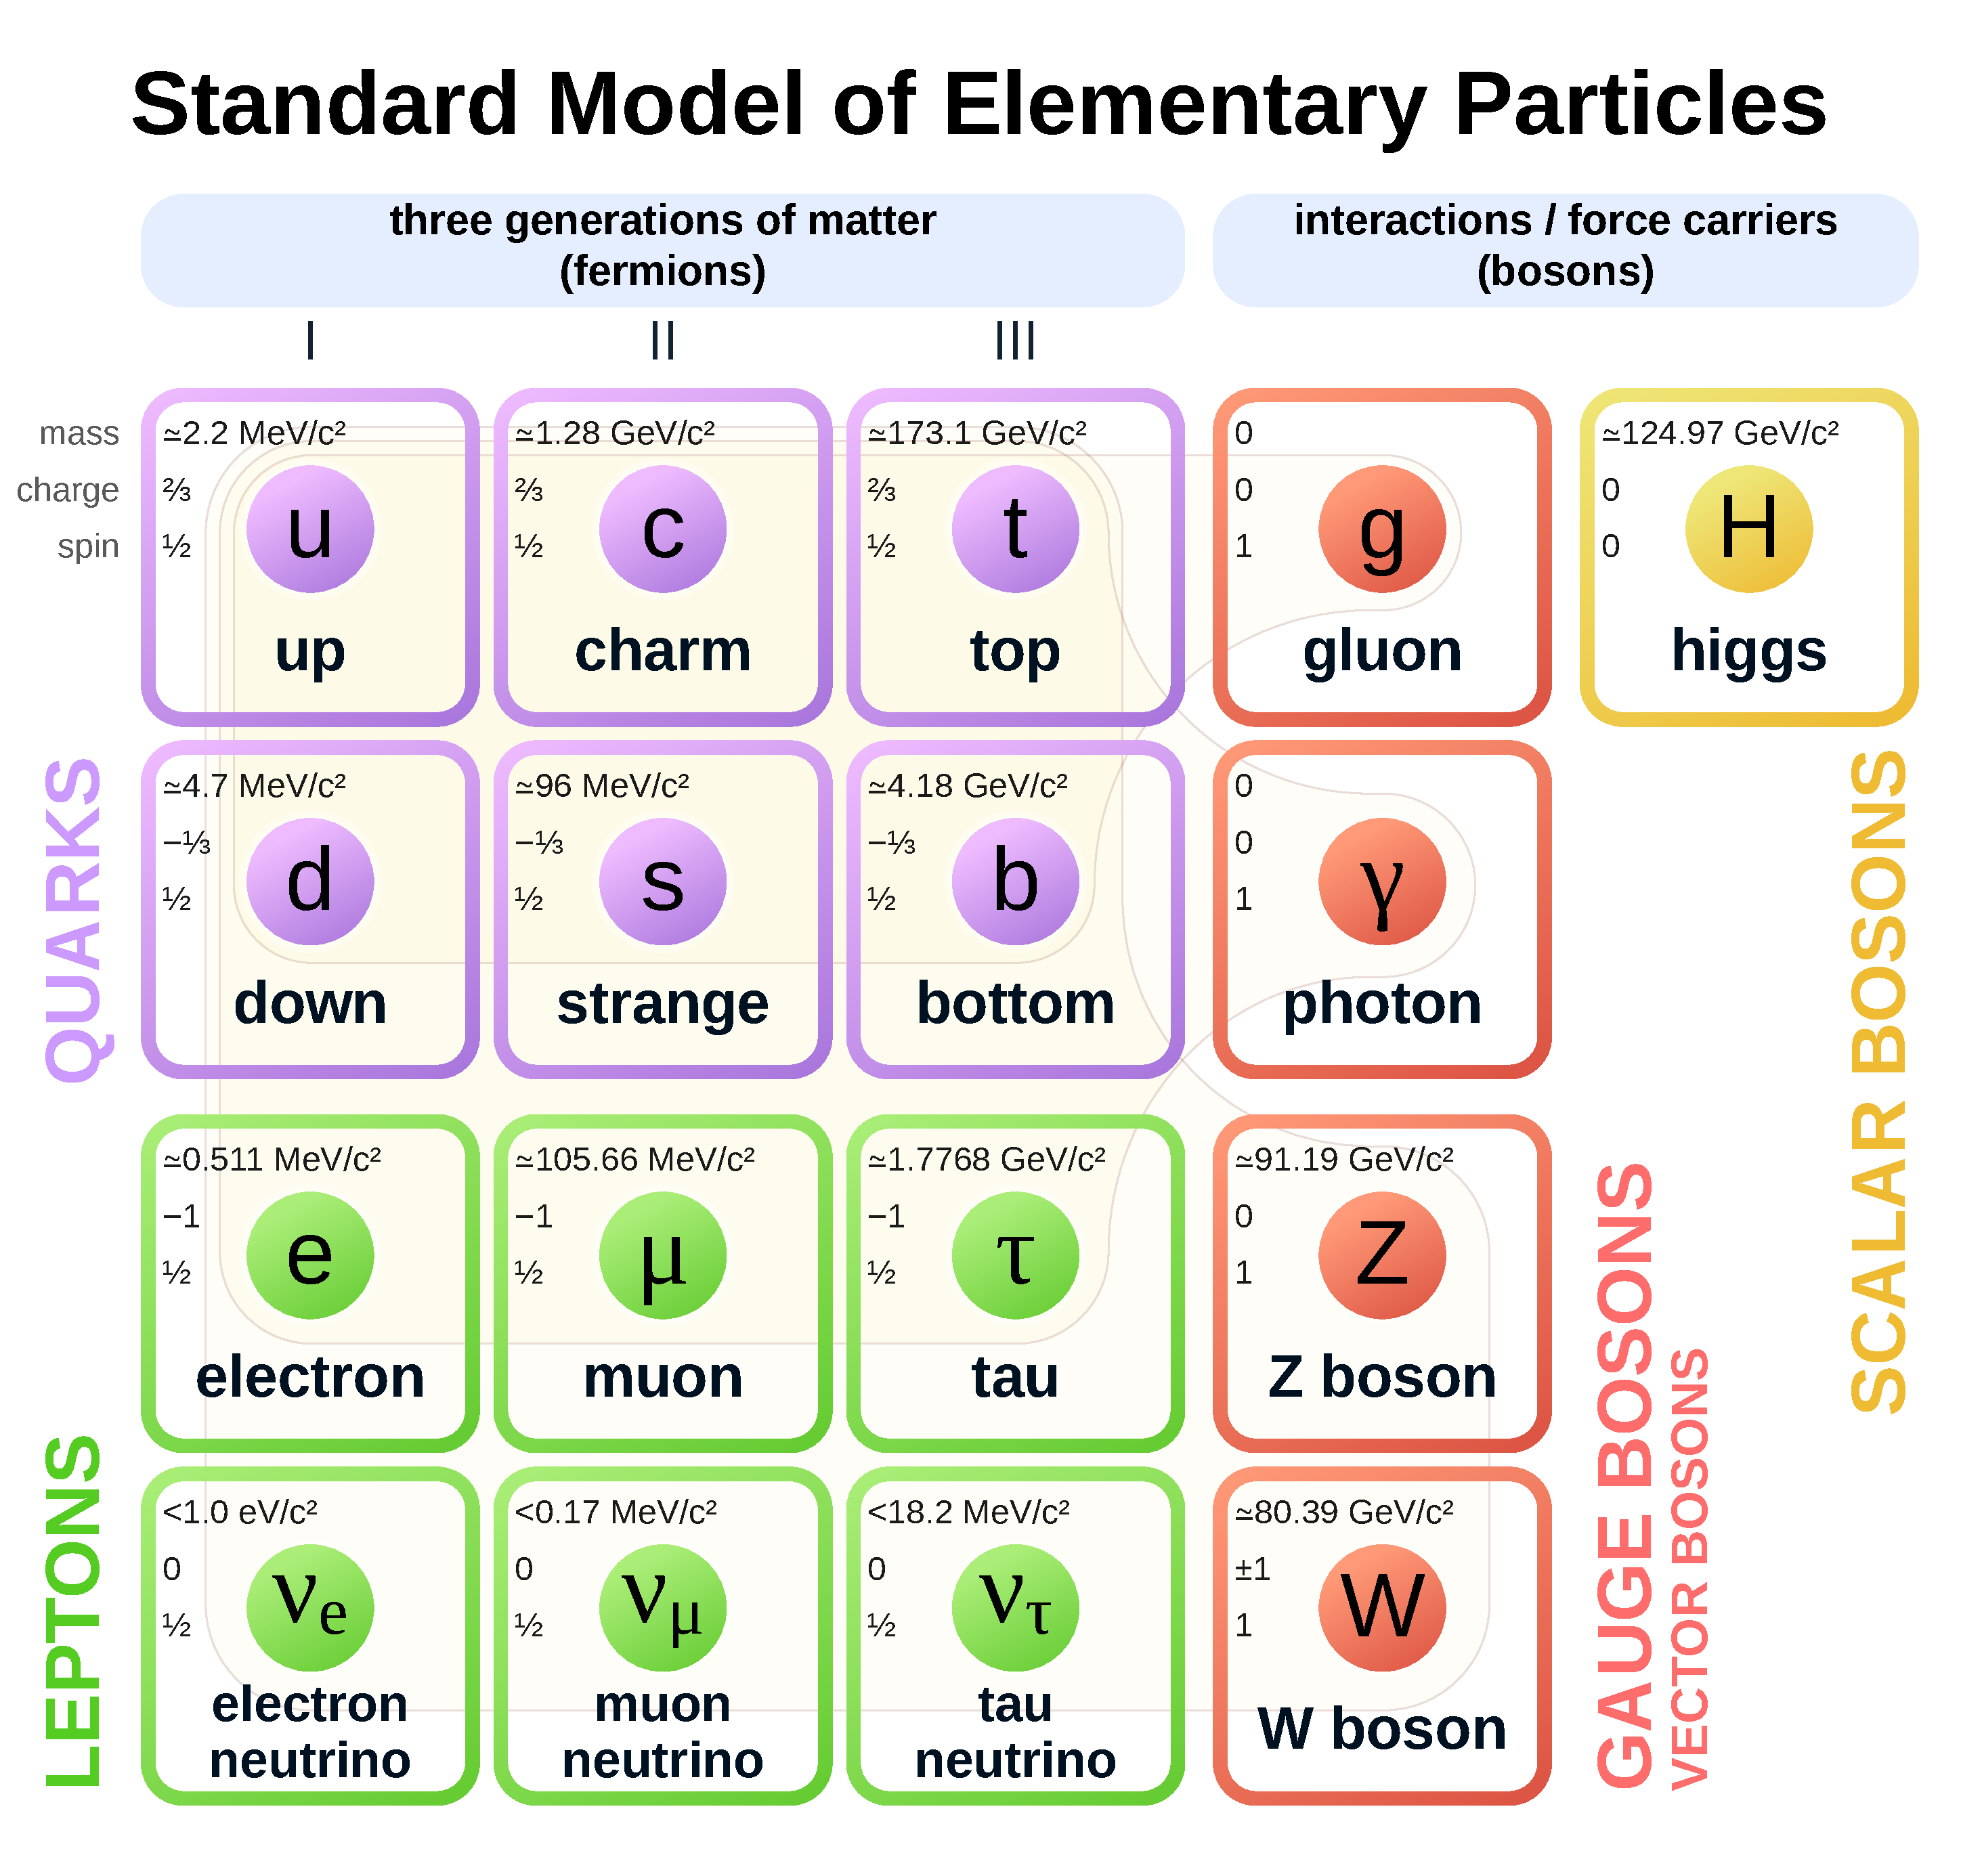
\includegraphics[width=\linewidth,height=\textheight,keepaspectratio]{theory/Standard_Model_of_Elementary_Particles}
        \caption{I'm probably going to need to find something else since this came from wikipedia. I just wanted a placeholder}
        \label{fig:sm_particles}
    \end{figure}

    There are twelve distinct elementary fermions (see Figure \ref{fig:sm_particles}),
        which are split evenly into two subgroups, called quarks and leptons.
    Quarks have a charge of 1 with the Strong Interaction,
        while leptons have a charge of 0 (and thus cannot interact via the Strong Interaction at all).
    Both classes of particles -- quarks and leptons -- are divided into three ``generations'' of progressively heavier particles.
    Each generation accordingly consists of two quarks and two leptons.
    These pairs, dubbed ``doublets'', behave the same across all generations.
    Among the quarks, every generation contains a doublet of an up-type quark (Up, Charm, Top) with electromagnetic charge of 2/3,
        and a down-type quark (Down, Strange, Bottom) with EM charge of -1/3.
    For leptons, each doublet consists of a charged particle (electron, muon, tauon) with EM charge of -1,
        and a chargeless neutrino with EM charge of 0.
    In addition to the fermions, there is also an entirely seperate class of particles, called gauge bosons,
        which play a fundamental role in the aforementioned interactions.
    However, an in-depth discussion of these particles will need to wait until Section \ref{sec:gauge_symmetry}.

    Mathematically, particles are described as pertubations of an overall ``quantum field.''
    A particle field $\varphi$, describes every particle of the same type at once,
        and particle states $\ket{\varphi}$ correspond to the number of that kind of particle that exists at a given moment.
    Fermions in particular are described as manifestations of ''Dirac Fields'', $\psi(x)$,
        which are defined as solutions to an equation of motion known as the Dirac Equation
    \begin{equation} \begin{split}
        (\gamma^\mu p_\mu - m) \psi(x) = 0
        \\ (i\gamma^\mu \partial_\mu - m) \psi(x) = 0
    \end{split} \end{equation}
    The term $\gamma^\mu$ is a vector of matrices, simply called the gamma matrices.
    The gamma matrices are a fascinating subject all their own, 
        but for the purposes of this discussion it will suffice to state that
        their primary function is in allowing the 4-vector $p_\mu$ to be added to the scalar $m$.

    As a final note on the topic of matter,
        I need to mention a peculiar consequence of Quantum Field Theory, in the form of \textit{anti-matter}.
    Anti-matter particle fields correspond to negative-energy solutions to the Dirac Equation,
        and are represented as
    \begin{equation}
        \psibar(x) \equiv \gamma^0 \psi\dag(x)
    \end{equation}
    Anti-matter particles are identical to their matter components in every way,
        with the most notable change being that their charges are inverted.

    The brilliance of the Standard Model lies in how it is able to describe the 
        particles and interactions of nature as consequences of pure mathematical structures.
    Describing matter in mathemetical form is the first step in constructing the Standard Model.
    The next step is to do the same with motion.


\section{Generating Motion: Group Theory and Transformations}

    %TODO Add a transistion here
    A function can be altered using a \textit{transformation operator}.
    A simple example of this would be a function $x(t)$, 
        which (assuming constant velocity) can be transformed into a time $\Delta t$ in the future as
    \begin{equation}
    x(t) \to x'(t) = x(t) + v \Delta t
    \end{equation}
    Recognizing that $v$ is just $\frac{d}{dt} x(t)$, this can be rewritten as
    \begin{equation}
    x(t) \to x'(t) = x(t) + \Delta t \frac{d}{dt} x(t) = \left(1+\Delta t \frac{d}{dt}\right) x(t)
    \end{equation}

    This term $\left(1+\Delta t \frac{d}{dt}\right)$ is the classical time-translation operator.
    Notice the assumption of constant velocity though.
    If velocity were not constant, this operator would be invalid, except in the specific case for which $\Delta t$ is infinitesimal.
    \begin{equation}
    x(t) \to x'(t) = \lim_{\delta t \to 0} \left(1+\delta t \frac{d}{dt}\right) x(t)
    \end{equation}

    To produce a more general finite operator I can apply the infinitesimal operator an infinite number of times
    \begin{equation} \begin{split}
    x(t) \to x'(t) &= \lim_{\delta t \to 0} \left(1+\delta t \frac{d}{dt}\right)\left(1+\delta t \frac{d}{dt}\right)\left(1+\delta t \frac{d}{dt}\right)...\ x(t)
    \\x(t) \to x'(t) &= \lim_{N \to \infty} \lim_{\delta t \to 0} \left(1+\delta t \frac{d}{dt}\right)^N x(t)
    \\x(t) \to x'(t) &= e^{\Delta t \frac{d}{dt}} x(t)
    \end{split} \end{equation}

    Where $\Delta t$ is again a finite time transformation,
        and I have compressed the infinite product of terms using the power series expansion of the exponential function.
    In order to use this classical operator in quantum field theory, it must have a complex factor `$i$' associated with it,
    \begin{equation} \begin{split}
    x(t) \to x'(t) = e^{i\Delta t \frac{d}{dt}} x(t)
    \end{split} \end{equation}

    Returning to Dirac Fields, which are functions of four-position $x_\mu$, this same transformation can be used
         with the minor adjustment of changing the total derivative to a partial derivative in time, $\frac{partial}{\partial t} = \partial_0$
    \begin{equation} \begin{split}
    \psi(x) \to \psi'(x) = e^{i\Delta x^0 \partial_0} \psi(x)
    \end{split} \end{equation}

    Meanwhile, the Dirac anti-particle field transforms with a negative sign as
    \begin{equation} \begin{split}
        \psibar(x) \to \psibar'(x) = e^{-i\Delta x^0 \partial_0} \psibar(x)
    \end{split} \end{equation}
    
    The time translation operator is but one of a myriad of different tranformation operators.
    However, all of the transformation operators used here take a similar form to this, appearing as
    \begin{equation} \begin{split}
        \psi(x) \to \psi'(x) = e^{ q \cdot \mathcal{F}_q } \psi(x)
    \end{split} \end{equation}
    $\mathcal{F}_q$ is the transformation \textit{generator} (e.g.\ $i\partial_0$),
        and $q$ the amount to transform by (e.g.\ $\Delta t$).

    These transforms fall under a larger realm of mathematics known as Group Theory,
        and are in turn called ``group transformation''.
    The basic definition of a group is a set of elements which can be ``multiplied'' according to some rule,
        and which satisfies the following four conditions\cite{Cheng_book}:
    \begin{itemize}
        \item Closure - the product of any two elements of the group are still in that group;
        \item Associativity - $(a \times b)\times c = a\times(b \times c)$;
        \item Identity - there is some element in the group $I$ for which $I \times a=a$;
        \item and Inversion - every element $a$ has an inverse $a^{-1}$ such that if $b \times a = c$ then $c \times a^{-1} = b$.
    \end{itemize}

    It should be relatively simple to see that time translation operations satisfy each of these.
    Additional classifications for groups are whether a group is discrete or continuous,
        and whether a group is ``Abelian'' (commutative) or ``non-Abelian'' (non-commutatitve).
    Time translations are continuous (one can tranlate by an infinitesimally small amount of time),
        and are Abelian (the order that the translation are applied does not matter).
    An example of a non-Abelian group would be that of three-dimensional rotations (formally called the $SO(3)$ group),
        as applying rotations in a different order can lead to a different final orientation.

    As a final point regarding Group Theory, is the absolutely crucial idea of \textit{symmetry}.
    If a system can be transformed under a group transformation and remain overall unchanged,
        then that system is said to be invariant, or symmetric, under that group.

    In a very deep sense, Group Theory and symmetry are the driving forces behind the entire Standard Model.
    Not only is the motion of the Standard Model entirely described by Group Theory,
        but as will be seen in the coming sections,
        its interactions are defined by Group Theory,
        and its entire organizational structure ultimately rooted in Group Theory.


\section{Restricting Motion: The Lagrangian and Symmetry}
    
    The Dirac Equation describes the equation of motion of a single field,
        but what is required is a way to describe the interactions of \textit{many} fields.
    For this, the Standard Model makes use of the Principle of Least Action,
        also known as the Lagrangian Formulation\cite{Halzen_book}.
    The idea of the Principle of Least Action is to construct an overall description of all aspects of a system,
        called the Lagrangian, $\Lag$.
    One can then find the ``path'' of this Lagrangian which minimizes the ``Action'', $\mathscr{A}$
    \begin{equation} %TODO: double check this!!
        \mathscr{A} = \int \Lag d^4 x
    \end{equation}

    This minimization is performed using the four-dimensional Euler-Lagrange equations
    \begin{equation}
        \partial_\mu \frac{\partial \Lag}{\partial_\mu \varphi } - \frac{\partial \Lag}{\partial \varphi} = 0
    \end{equation}
    which yields the equations of motion of the interacting particles.

    All of the physics of the Standard Model is inscribed within the Standard Model Lagrangian.
    The construction of this Lagrangian will be the focus of most of the rest of the chapter.
    To begin then, what physics \textit{does} the Lagrangian need to encode?
    Paraphrasing Murray Gell-Mann, ``that which is not forbidden, is \textit{mandatory}.''
    That is to say, that any physics which is not expressly prohibited, can and will occur.
    Formulation of the Standard Model Lagrangian must therefore start with an enumeration of restrictions,
        which are given in the form of a series of groups that the Lagrangian must remain symmetric under.
    Specifically, the Lagrangian must remain symmetric under ten transformations,
        collectively referred to as the Poincare Group.
    Four of these transformations correspond to the space-time translations,
        three to spatial rotations, and the remaining three to space-\textit{time} rotations,
        also known as Lorentz Transformations (also known as just changing velocity).

    The Lagrangian of a Dirac field satisfying these symmetries takes the form
    \begin{equation} \label{eq:basic_fermionL}
        \Lag = \psibar (\gamma^\mu p_\mu - m) \psi = i \psibar \gamma^\mu \partial_\mu \psi - m \psibar \psi
    \end{equation}
    As an example of the symmetry now described, I will reuse the time translation operator $e^{i\Delta x^0 \partial_0}$

    \begin{equation} \begin{split}
        \Lag(t) \to \Lag' = \Lag(t+\Delta t) =
            \left( e^{-i\Delta x^0 \partial_0} \psibar \right) (\gamma^\mu p_\mu - m) \left( e^{i\Delta x^0 \partial_0}\psi \right)
        \\  = e^{-i\Delta x^0 \partial_0 + i \Delta x^0 \partial_0} \psibar (\gamma^\mu p_\mu - m) \psi
        \\  = \psibar (\gamma^\mu p_\mu - m) \psi
    \end{split} \end{equation}

    Applying the Euler-Lagrange equations to this equation will seperately return the Dirac Equation
        for the fermion and anti-fermion fields, as it should.

    Given that there are many different kinds of fermions, the Lagrangian can be expanded to include all of them
    \begin{equation}
        \Lag = \bar{e} (\gamma^\mu p_\mu - m) e
        + \bar{\mu} (\gamma^\mu p_\mu - m) \mu
        + \bar{\tau} (\gamma^\mu p_\mu - m) \tau
        + \bar{u} (\gamma^\mu p_\mu - m) u
        + ...
    \end{equation}

    Although this equation qualifies as a valid description of the motion of fermions,
        there is a glaring flaw with it: the fields it describes are all completely independent of one another.
    In its current form, the Lagrangian proposes that particles, given some initial momentum,
        will persist along the same trajectory forever, unable to affect or be affected by any other particle.
    The Lagrangian has succesfully constrained the range of allowed physics,
        but it has done so to such a degree that the described physics are now practically static.
    Clearly, this is not a satisfactory description of the universe, full of dynamic interactions as it is.
    The resolution to this issue is, counter-intuitively, to enforce yet \textit{more} symmetry requirements.
    In doing so, the various interactions of the Standard Model will be laid bare,
        and the beauty of the theory made apparent.

    %Should I also discuss renormalizability? (Peskin pg 80/101djvu)
    %Basically, all lagrangians must be renormalizable.
    %Renormalizability just means that the lagrangian doesn't explode from the unconstrained nature of virtual particles.
    %So infinite-mass virtual particles should not break a renormalizeable lagrangian.


\section{Transferring Motion: Gauge Symmetry} \label{sec:gauge_symmetry}

    %Describe Global U1
    Allow me to introduce another group, called $U(1)$ (Unitary Rank 1 Group).
    This group corresponds to the phase of a field, and the transformation takes the form
    \begin{equation}
        \psi(x) \to \psi'(x) = e^{i\theta} \psi(x)
    \end{equation}

    %describe global vs local
    As in prior examples, the exponential changes signs for the anti-fermion.
    The generator here is just $i$, the phase shift amount given by the angle $\theta$.
    It is trivial to see that the Lagrangian is invariant under such a group.
    This transformation, along with all the others already described under the Poincare group,
        all fall under the category of \textit{global} transformations.
    A global transformation is one which is applied uniformly across all of space-time.
    There is a different kind of transformation, called a Local or ``Gauge'' transformation.
    Gauge transforms are such that the transformation amount varies \textit{at each point in space-time}.
    A local $U(1)$ transform would thus take the form 
    \begin{equation}
        \psi(x) \to \psi'(x) = e^{i\theta(x)} \psi(x)
    \end{equation}
    Noting that the phase-angle $\theta(x)$ is now a function of $x$.

    Demanding that the Lagrangian remain invariant under such a transformation would surely be an absurd mandate.
    Nonetheless, this is exactly what nature seems to have done.

    %Show how this breaks lagrangian
    I want to show how the Lagrangian in its current form breaks when attempting to perform a $U(1)$ gauge transform,
        and how the resolution to this issue leads directly to fully dynamic, interacting Lagrangian.
    First, apply the gauge transformation
    \begin{equation} \begin{split}
        \Lag(\theta_0) \to \Lag' = \Lag(\theta_0+\theta(x)) &=
            \left( e^{-i\theta(x)} \psibar \right) (\gamma^\mu p_\mu - m) \left( e^{i\theta(x)}\psi \right)
            \\ &= \left( e^{-i\theta(x)} \psibar \right) i\gamma^\mu \partial_\mu \left( e^{i\theta(x)}\psi \right)
                - \left( e^{-i\theta(x)} \psibar \right) m \left( e^{i\theta(x)}\psi \right)
    \end{split} \end{equation}
    In the mass term, the transform will cancel in the usual fashion.
    The momentum term however will \textit{not} cancel, as the derivative will also affect the position-dependant $\theta(x)$.
    \begin{equation} \begin{split}
        \Lag' &= \left( e^{-i\theta(x)} \psibar \right) i\gamma^\mu \partial_\mu \left( e^{i\theta(x)}\psi \right) - m \psibar(x) \psi(x)
        \\ &= i \left( e^{-i\theta(x)} \psibar \right) \left[
                \left( \gamma^\mu \partial_\mu e^{i\theta(x)} \right) \psi 
                + e^{i\theta(x)} \left( \gamma^\mu \partial_\mu \psi \right)
            \right] - m \psibar(x) \psi(x)
        \\ &= i \left( e^{-i\theta(x)} \psibar \right)
                \left( \gamma^\mu \partial_\mu e^{i\theta(x)} \right) \psi 
            + i \psibar \gamma^\mu \partial_\mu \psi
            - m \psibar(x) \psi(x)
        \\ &= - \psibar \left( \gamma^\mu \partial_\mu\theta(x) \right) \psi 
            + \psibar ( \gamma^\mu p_\mu - m ) \psi
    \end{split} \end{equation}

    %Show how to fix lagrangian
    Under a local $U(1)$ transform, the Lagrangian is clearly not invariant,
        as a result of the additional $\gamma^\mu \partial_\mu\theta(x)$ term.
    In order to enforce gauge symmetry, a subtle but profound adjustment must be made to the Lagrangian.
    This adjustment will take the form of a modification to the derivative,
        replacing the standard derivative with a \textit{covarient} derivative,
    \begin{equation}
        \partial_\mu \to D_\mu \equiv \partial_\mu + i \emc A_\mu(x)
    \end{equation}
    where $\emc$ is a constant and the new function $A_\mu(x)$ is formulated such that it transforms under a $U(1)$ gauge rotation as
    \begin{equation}
        A_\mu(x) \to A'_\mu(x) = A_\mu(x) - \frac{1}{\emc} \partial_\mu \theta(x)
    \end{equation}

    With this additional term, the Lagrangian becomes
    \begin{equation} \begin{split}
    \Lag = \psibar (i\gamma^\mu D_\mu - m) \psi
        = \psibar \left[i\gamma^\mu(\partial_\mu + i \emc A_\mu) - m\right] \psi
    \end{split} \end{equation}
    and the specific transformation property of $A$ renders the entire equation invariant under a gauge transform
    \begin{equation} \begin{split}
    \Lag(\theta_0) \to \Lag' &= \Lag(\theta_0+\theta(x))
        \\&= \left( e^{-i\theta(x)} \psibar \right) 
        \left[i\gamma^\mu \left(\partial_\mu 
            + i \emc \left[A_\mu - \frac{1}{\emc} \partial_\mu \theta(x)\right] \right) 
            - m\right]
        \left( e^{i\theta(x)}\psi \right)
        \\&= \psibar \left[i\gamma^\mu(\partial_\mu + i \emc A_\mu) - m\right] \psi
    \end{split} \end{equation}

    % Introduce photon field and show newly produced interaction
    % See Peskin pg484 (djvu 505) for derivation of kinetic term
    % See also https://physics.stackexchange.com/questions/131097/gauge-field-tensor-from-wilson-loop
    Through a much more sophisticated derivation (which will not be demonstrated here),
        it can also be shown that this new covarient derivative causes the Action to acquire an additional term 
        related to the commutator of the covarient derivative, $[D_\mu, D_\nu] \equiv D_\mu D_\nu - D_\nu D_\mu$.
    Defining a tensor $F_{\mu\nu}$ as $i\emc F_{\mu\nu} = [D_\mu, D_\nu]$,
        the additional required term takes the form $-\frac{1}{4}F^{\mu\nu}F_{\mu\nu}$.
    The final expression for the $U(1)$ gauge invariant fermion Lagrangian now appears as
    \begin{equation} \label{eq:qedL} \begin{split}
        \Lag &= \psibar (i\gamma^\mu D_\mu - m) \psi - \frac{1}{4}(F_{\mu\nu})^2
        \\&= i \psibar \gamma^\mu \partial_\mu \psi
            - m \psibar \psi
            + i \emc \psibar \gamma^\mu A_\mu \psi
            - \frac{1}{4}F_{\mu\nu}F^{\mu\nu}
    \end{split} \end{equation}

    Of extraordinary note is that the last term of $\Lag$ is completely independant of the Dirac field $\psi$.
    The true nature of $A$ is thus revealed, not as just a mere correction factor,
        but as a massless field all its own.
    Indeed, $A(x)$ corresponds to the photon field, $\emc$ to the electric charge,
        and the term $-\frac{1}{4}(F_{\mu\nu})^2$ to the kinitec energy of the photon.
    Furthermore, the three-field term $i \emc \psibar \gamma^\mu A_\mu \psi$
        allows the Dirac field to interact directly with the photon field,
        and through the photon field to interact indirectly with \textit{other} Dirac fields.
    Far from the static situation described by Equation \ref{eq:basic_fermionL},
        the new Lagrangian permits a wide range of dynamic interactions between particles.
    In fact, using the Euler-Lagrange equations on Equation \ref{eq:qedL}
        will now reproduce the Lorentz Force Law as the equation of motion for the Dirac fields,
        and Maxwell's Equations as the equation of motion for the photon.

    % Introduce SU(2) and SU(3)
    All of this complexity arose from the simple imposition of the $U(1)$ gauge symmetry upon the fermion Lagrangian.
    The full extent of interaction in the Standard Model can be realized by imposing then two more gauge group symmetries:
        $SU(2)$, and $SU(3)$.
    Both of these groups behave in a similar manner to $U(1)$, with the transformations taking the forms
    \begin{equation} \begin{split}
        SU(2)&: e^{i \alpha^a(x) \sigma^a / 2}
        \\SU(3)&: e^{i \xi^b(x) \mathscr{F}^b / 2}
    \end{split} \end{equation}
    where $\sigma^a$ corresponds to the three, 2x2 Pauli Matrices
    \begin{equation}
        \sigma^1 = \begin{pmatrix} 0 & 1 \\ 1 & 0 \end{pmatrix} \quad
        \sigma^2 = \begin{pmatrix} 0 & -i \\ i & 0 \end{pmatrix} \quad
        \sigma^3 = \begin{pmatrix} 1 & 0 \\ 0 & -1 \end{pmatrix}
    \end{equation}
    and $\mathscr{F}^b$ corresponds to the eight, 3x3 structure constant matrices of $SU(3)$
        (which don't have a formal name and will not be explicitly written out).

    While $U(1)$ acted as one-dimensional rotation of a single complex angle $\theta$,
        $SU(2)$ performs three orthogonal rotations $\alpha^a$ through a three-dimensional complex space,
        and $SU(3)$ performs rotations through an eight-dimensional complex space.
    Because $SU(2)$ operates through the 2x2 Pauli Matrices, it must operate on the fermions as ``doublets''
        (recall Section \ref{sec:standard_model}).
    \begin{equation}
        \minimatrix{u_L \\ d_L} \to e^{i \alpha^a \sigma^a / 2} \minimatrix{u_L \\ d_L}
    \end{equation}

    Similarly, the triplet nature of $SU(3)$ neccesitates that the group operate on all three generations of fermions at once
    \begin{equation}
        \minimatrix{u\\c\\t} \to e^{i \xi^b \mathscr{F}^b / 2} \minimatrix{u\\c\\t}
    \end{equation}

    Neither group operates uniformly across the fermions though.
    $SU(2)$ acts only on the ``left-handed'' chiral state of the fermions (denoted by the subscript L),
        and $SU(3)$ acts only on the quarks, having a charge of zero for all leptons.

    The behaviour of these Gauge Groups established, the natural assumption is that the three gauge fields
        $U(1)$, $SU(2)$, and $SU(3)$ correspond to the three fundamental interactions,
        Electromagnetic, Weak, and Strong.
    This would serve to complete a theory of the universe based entirely on the geometric principle of symmetry.
    $SU(3)$ assuredly does correspond to the strong interaction, its gauge field manifested as the Gluons.
    Likewise, the electromagnetic interaction and its photons have already been revealed as manifestation of the $U(1)$ group. 
    All of this breaks down however with $SU(2)$, which does \textbf{not} correspond to the W and Z bosons;
        at least, not directly.

    The problem is that the W and Z fields have mass.
    Gauge fields \textit{cannot} have mass.
    A brief check will confirm that a lagrangian mass term such as $m_Z^2 (Z^0)^2$
        will not remain invariant under the gauge field's own tranformation.
    By all rights, the experimental measurement of the W and Z masses should have
        ended the idea of gauge symmetry as a principle of nature altogether.
    Instead, a theory was proposed which would allow gauge symmetry to persist,
        but only under the condition that an entirely new field, unlike any previously observed, must exist.
    Not only did this theory resolve the origin of the W and Z masses;
        it predicted -- nearly a half-century in advance of its discovery --
        the existance of the scalar particle now known as the Higgs Boson.
    \cite{Osborn_notes}
    \cite{Peskin_book}
    \cite{Halzen_book}

